\chapter{Implementierung}

\section{Architekturentscheidungen}

Zugrundeliegend: Gemeinsamkeit von Protokollen, Erweiterbarkeit/Pluginfähigkeit, ...

Warum Java? (UHH als Einstieg-> für alle verständlich und auch erweiterbar, ...)

Welche TLS-Version? Oder SSL 2.0? Aus welchen Gründen? (1.2, aktuell, demonstriert Funktionsweise und Verhinderung von Angriffen; zum \inquotes{Durchklicken} von Angriffen wäre SSL schöner, ...)

Welche Dinge werden betrachtet, welche ausgelassen (Extensions, Zertifikatvalidierung, ...), aus welchen Gründen?

Ausgelassen:
\begin{itemize}
\item TLS-Extensions
\item Zertifikatsvalidierung, PKI und Verwandtes
\item Komprimierung
\item eingeschränkte Anzahl von CipherSuites (und Schlüsselaustausch)
\item Ältere Versionen
\item Clientauthentifizierung
\item Fragmentierung oder mehrere TlsMessages in einem Record
\end{itemize}

\section{Implementation notes}

Analyse (Rückgriff auf Didaktik-Kapitel), Entwurf (UML ist toll, Automatenmodelle, ...), Implementierung, Tests, Evaluation...

Probleme/Schwierigkeiten bei der Umsetzung, ...

\begin{figure}[H]
	\centering
	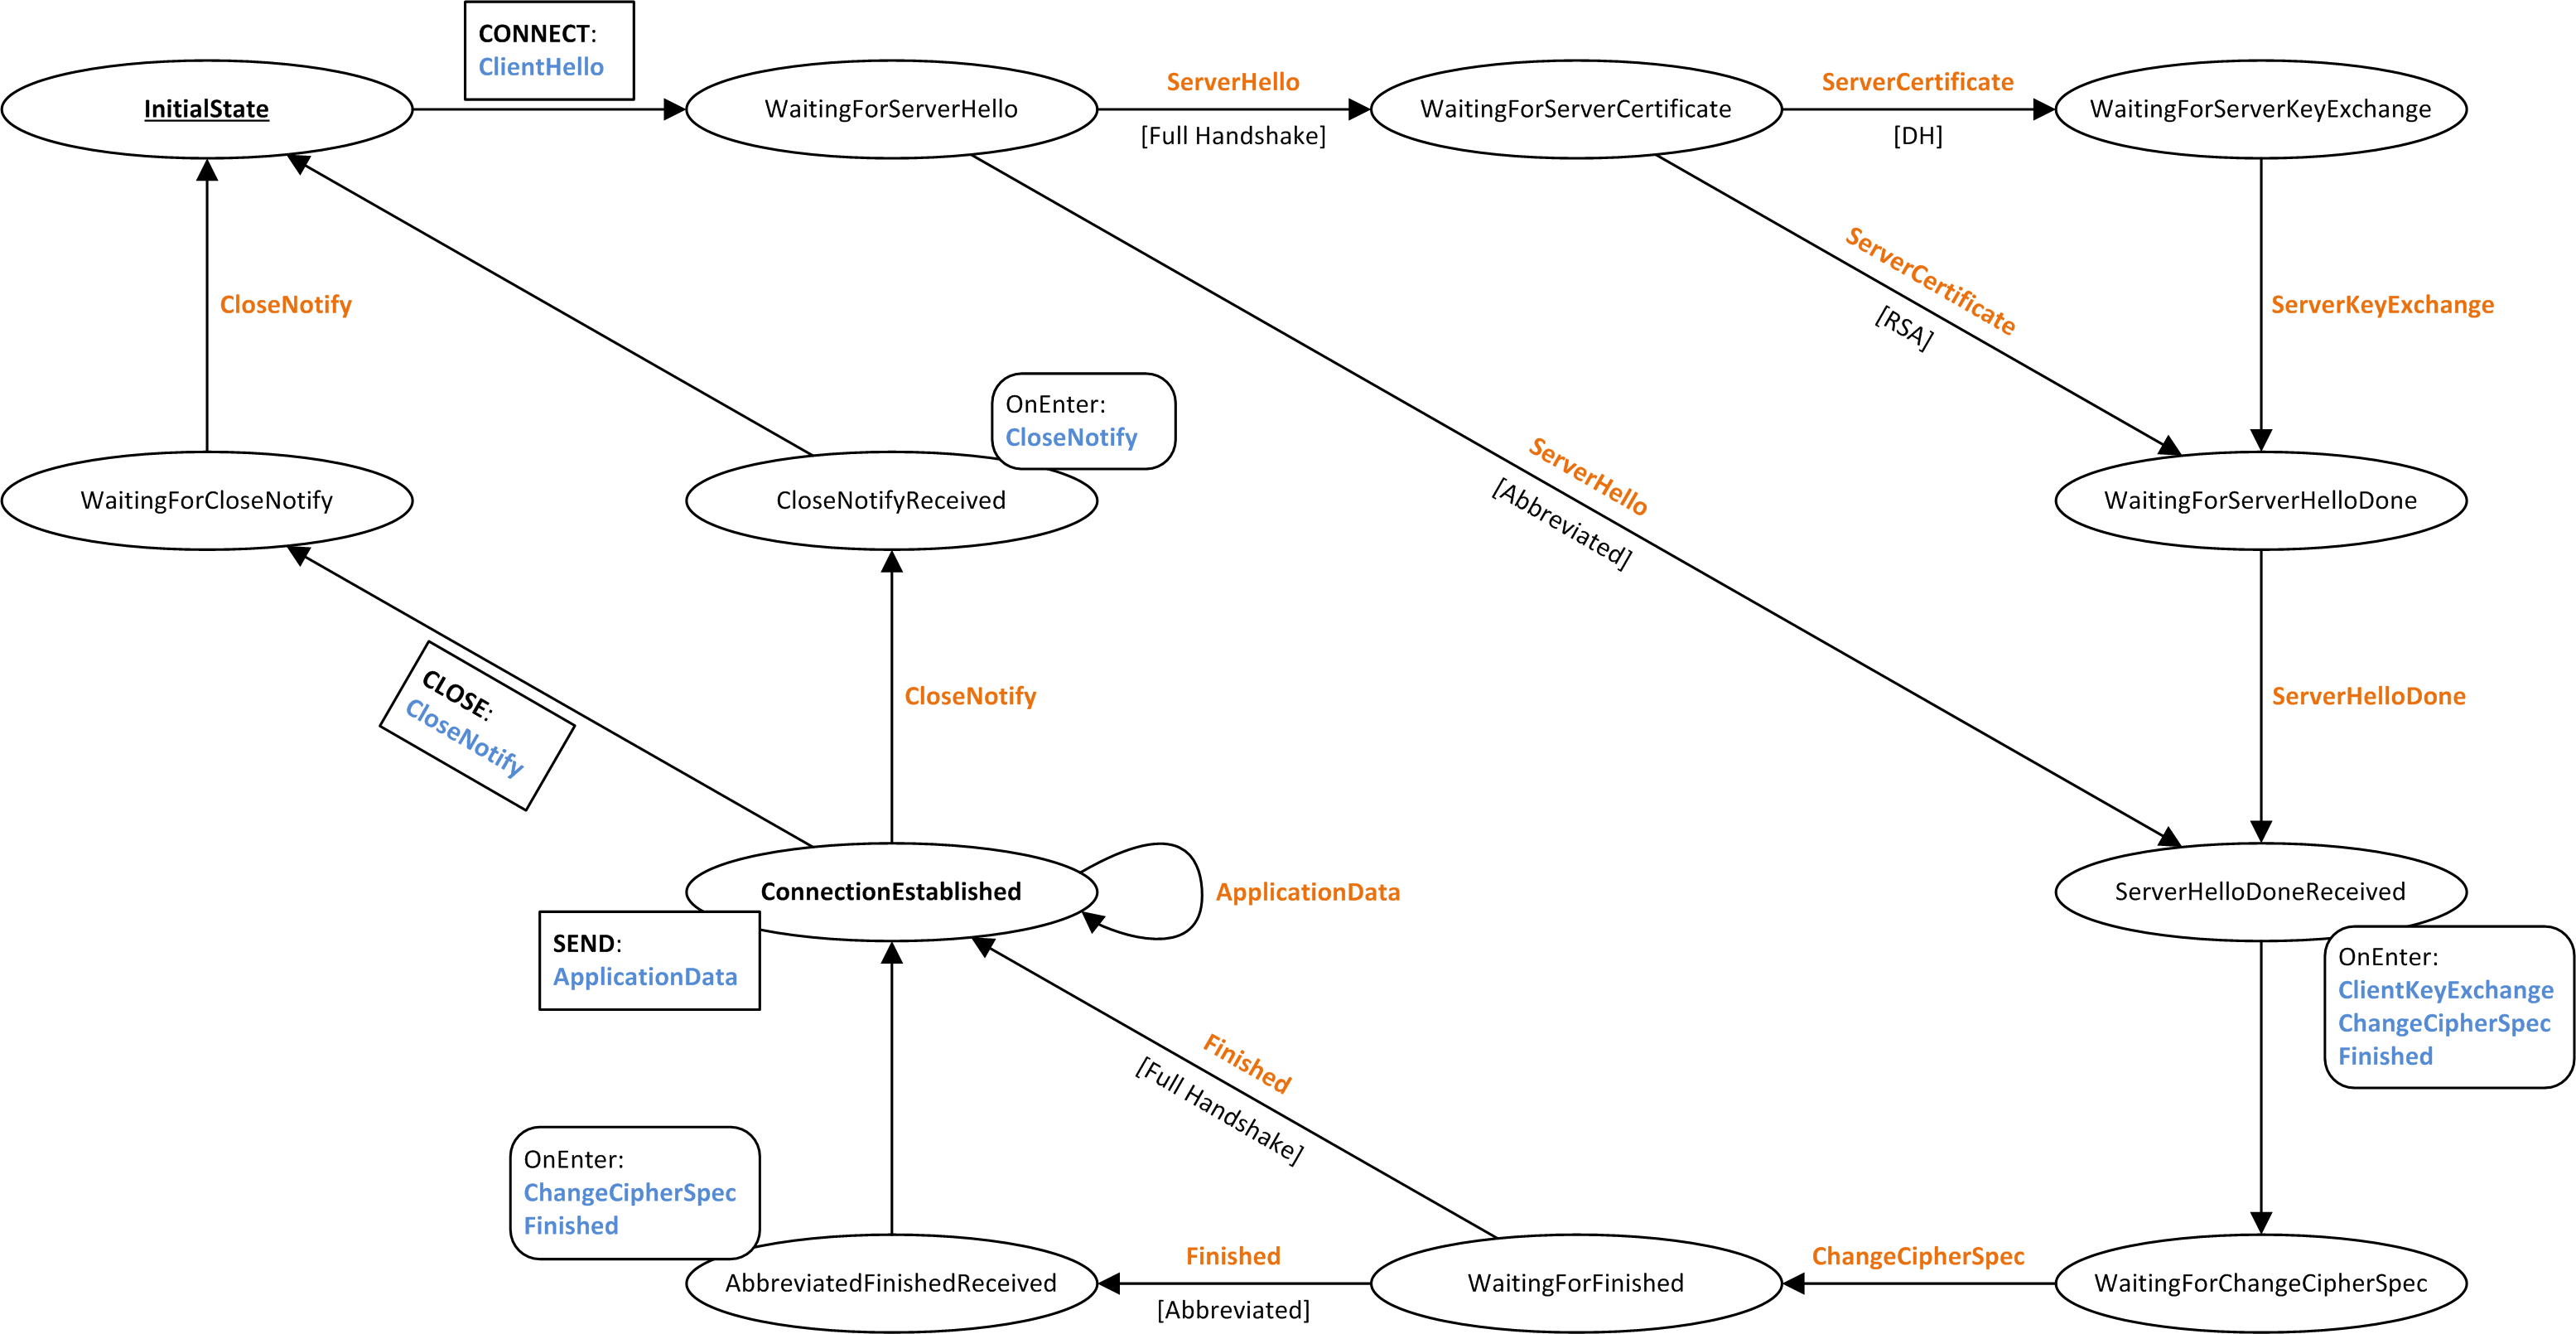
\includegraphics[scale=0.75, angle = 90]{Diagrams/client_state_machine.png} %
	\caption{Der Automat für den TLS-Client}
	\label{fig_tls_client_state_machine}
\end{figure}

\begin{figure}[H]
	\centering
	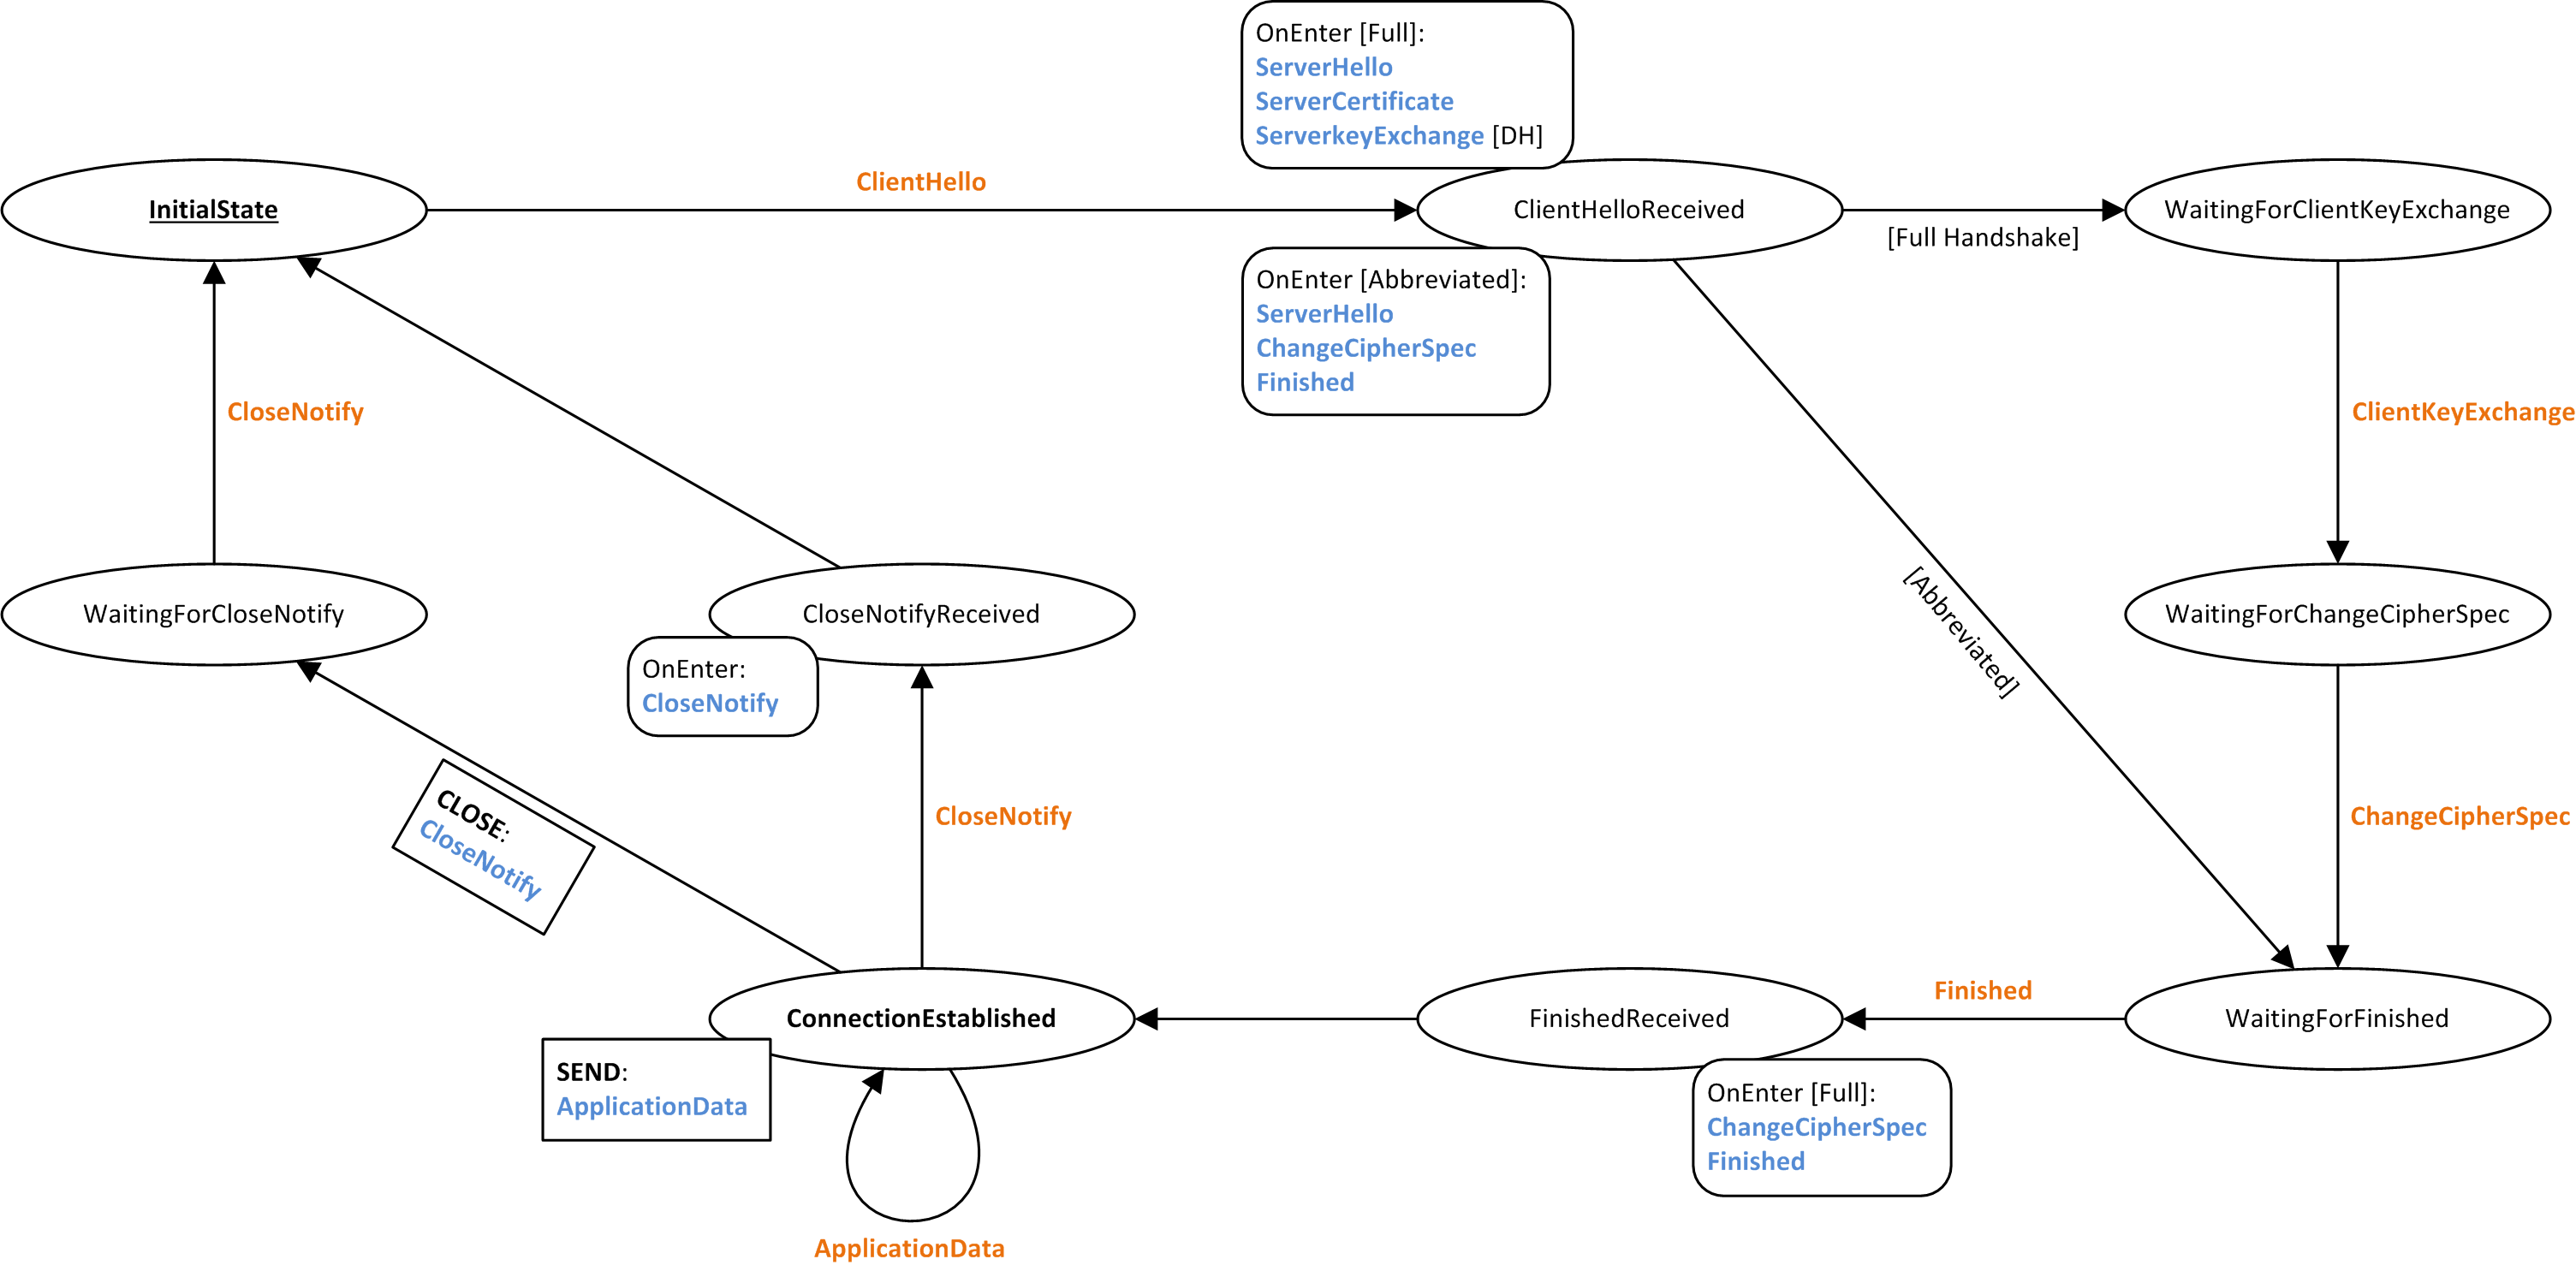
\includegraphics[scale=0.75, angle = 90]{Diagrams/server_state_machine.png} %
	\caption{Der Automat für den TLS-Server}
	\label{fig_tls_server_state_machine}
\end{figure}

\section{Tutorial: So schreibe ich ein Plugin, ...}

Evtl. auch in den Anhang?